\section{Model Details}
\label{app:model}

\subsection{Inputs}

Table~\ref{tab:inputs} lists the activity durations with their sources; all durations are lognormal with the stated mean and coefficient of variation (CV) and are sampled once per patient, so they do not depend on the policy. The acuity mixes, admission probabilities and CTAS targets are given in Table~\mref{tab:parameters}. Fig.~\ref{fig:profile} shows the hourly arrival profile (normalized to mean one; it ranges from \ProfileMin{} to \ProfileMax) and the boundaries of the three physician shifts.

\begin{table}[!htbp]
\centering
\caption{Activity durations (minutes; lognormal) and sources. ``Assumption'' marks values without a published source.}
\label{tab:inputs}
\footnotesize
\begin{adjustbox}{max width=\linewidth}\begin{tabular}{lrrp{6.6cm}}
\toprule
Activity & Mean (min) & CV & Source \\
\midrule
Physician initial assessment & 40/30/25/18/12 & 0.6 & assumption (longer for higher acuity) \\
Triage & 6 & 0.5 & assumption \\
Registration (delay) & 5 & 0.5 & assumption (delay, no resource) \\
Physician reassessment & 12 & 0.6 & assumption \\
Laboratory (LB) & 60 & 0.5 & assumption (laboratory turnaround) \\
X-ray (XR) & 25 & 0.5 & assumption (including transport) \\
CT & 35 & 0.5 & assumption (including transport) \\
Consultation (DR) & 60 & 0.7 & assumption (consultant arrival and assessment) \\
Discharge process & 15 & 0.6 & assumption \\
Boarding, low & 180 & 1.0 & assumption informed by provincial median waits for an inpatient bed (Alberta 3.6 h, Ontario 7 h, 2022/23; Li2023\_EDOvercrowdingCADTH) \\
Boarding, high & 480 & 1.0 & assumption informed by the same figures (upper level) \\
\bottomrule
\end{tabular}\end{adjustbox}
\end{table}

\begin{figure}[!htbp]
\centering
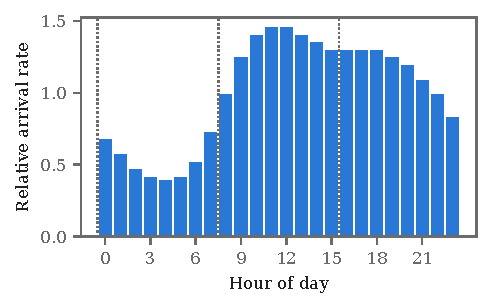
\includegraphics[width=0.8\columnwidth]{figures/fig_arrival_profile.pdf}
\caption{Hourly arrival profile (relative to the daily mean). Dotted lines: start of the night, day and evening physician shifts.}
\label{fig:profile}
\end{figure}

\subsection{Pathways}

Table~\ref{tab:pathways} lists the \NPathways{} published pathways \cite{Rismanchian2023_PatientJourney} with their published shares and the probability that a patient of a given CTAS level and disposition follows each of them in the model (typical diagnostic intensity). The probability of pathway $j$ for a patient of CTAS level $l$ with disposition $a$ is proportional to $f_j\exp\{(\theta_l+s)k_j\}$ over the pathways that end in $a$, where $f_j$ is the published frequency, $k_j$ the number of diagnostic and consultation steps, $\theta_l$ the CTAS tilt (from \TiltOneAll{} for CTAS~1 to \TiltFiveAll{} for CTAS~5) and $s$ the diagnostic-intensity shift.

\begin{table}[!htbp]
\centering
\caption{Published pathways and model probabilities by CTAS level, given the disposition in which the pathway ends (typical diagnostic intensity). TR triage, RG registration, AS physician assessment, LB laboratory, XR X-ray, DR consultation, DD discharge, AD admission.}
\label{tab:pathways}
\footnotesize
\begin{adjustbox}{max width=\linewidth}\begin{tabular}{llrrrr}
\toprule
 & & Published & \multicolumn{3}{c}{Model probability given disposition (\%)} \\
\cmidrule(lr){4-6}
Pathway & Steps & share (\%) & CTAS 1 & CTAS 3 & CTAS 5 \\
\midrule
V1 & TR-RG-AS-DD & 31.0 & 21.0 & 37.6 & 54.8 \\
V2 & TR-RG-AS-XR-DD & 16.0 & 17.9 & 19.4 & 17.1 \\
V3 & TR-RG-AS-LB-XR-DD & 10.9 & 20.1 & 13.2 & 7.1 \\
V4 & TR-RG-AS-CT-XR-DR-AD & 10.2 & 74.0 & 57.6 & 37.8 \\
V5 & TR-RG-AS-DR-DD & 10.1 & 11.3 & 12.2 & 10.8 \\
V6 & TR-RG-AS-LB-XR-DR-DD & 6.0 & 18.3 & 7.3 & 2.4 \\
V7 & TR-RG-AS-LB-AD & 4.1 & 11.0 & 23.2 & 41.4 \\
V8 & TR-RG-AS-XR-LB-AD & 3.4 & 15.0 & 19.2 & 20.8 \\
V9 & TR-RG-AS-LB-DD & 3.3 & 3.7 & 4.0 & 3.5 \\
V10 & TR-RG-AS-XR-LB-DD & 2.7 & 5.0 & 3.3 & 1.8 \\
V11 & TR-RG-AS-CT-DD & 2.4 & 2.7 & 2.9 & 2.6 \\
\bottomrule
\end{tabular}\end{adjustbox}
\end{table}

\subsection{Capacity Sizing and Load}

Let $\lambda_s$ be the arrival rate in shift $s$ at the base volume, and $\omega^{\text{hi}}$ and $\omega^{\text{lo}}$ the expected physician work per arriving patient contributed by CTAS~1--3 and CTAS~4--5 patients. The number of physicians in shift $s$ is
\begin{equation}
c_s=\big\lceil\lambda_s\omega^{\text{hi}}/\rho\big\rceil+\big\lceil\lambda_s\omega^{\text{lo}}/\rho\big\rceil,\qquad \rho=\PhysTargetMedium,
\end{equation}
and the second term is the fast-track team in the fast-track configuration. Treatment spaces are sized in the same way from the expected service-only holding time with $\rho=\SpaceSizing$, at the arrival rate that gives the medium load, and the CTAS~4--5 share forms the second area in the two-area configurations. Diagnostic resources are sized for an offered load of \DiagTarget{} and triage nurses for \TriageTarget{} at the busiest hour of the high load level. Finally the arrival rate is scaled so that the offered load of the busiest physician pool equals the load level (for the fast-track configuration, the larger of the Main and fast-track offered loads under CTAS streaming). Sensitivity and robustness experiments change demand-side inputs but keep these capacities.

\begin{table*}[!htbp]
\centering
\caption{Visits per day by load level, treatment spaces and physicians per shift (night/day/evening) for each acuity mix and configuration. Values in parentheses are the second area's share.}
\label{tab:capacity}
\footnotesize
\setlength{\tabcolsep}{5pt}
\begin{adjustbox}{max width=\linewidth}\begin{tabular}{llrrrrr}
\toprule
 & & \multicolumn{3}{c}{Visits per day} & Spaces & Physicians \\
\cmidrule(lr){3-5}
Acuity mix & Configuration & Low & Medium & High & (second area) & per shift (second area) \\
\midrule
Tertiary & Pooled & 229 & 262 & 295 & 41 & 4/10/9 \\
 & Fast track & 209 & 239 & 269 & 41 (5) & 4/10/9 (1/2/2) \\
 & Split flow & 229 & 262 & 295 & 41 (5) & 4/10/9 \\
\addlinespace
Community & Pooled & 218 & 249 & 280 & 35 & 4/9/7 \\
 & Fast track & 211 & 242 & 272 & 35 (9) & 4/9/7 (1/3/2) \\
 & Split flow & 218 & 249 & 280 & 35 (9) & 4/9/7 \\
\addlinespace
Urgent-care-like & Pooled & 233 & 267 & 300 & 31 & 4/8/7 \\
 & Fast track & 229 & 261 & 294 & 31 (15) & 4/8/7 (2/4/4) \\
 & Split flow & 233 & 267 & 300 & 31 (15) & 4/8/7 \\
\bottomrule
\end{tabular}\end{adjustbox}
\end{table*}

\subsection{Designs of the Robustness Experiments}

In E8 one input of a medium-load core ED type is changed at a time while all capacities stay as sized for the core inputs: physician activity times are multiplied by 0.9 or 1.1, diagnostic activity times by 0.75 or 1.25, every coefficient of variation by 0.5 or 1.5; the hourly arrival profile is replaced by a flat profile or by the core profile raised to the power 1.5 and renormalized (more peaked); or the predicted codes of a patient are drawn from one common uniform random number for all attributes, so that prediction errors are fully correlated across attributes.

In E9 the \NOosTypes{} ED types are drawn by Latin hypercube sampling in four dimensions, ten per configuration: an acuity position $t\in[0,1]$, which interpolates the CTAS shares linearly between the urgent-care-like ($t=0$), community ($t=0.5$) and tertiary ($t=1$) mixes; the offered load of the busiest physician pool in $[0.70,0.90]$; the mean boarding time in $[120,360]$ minutes; and a shift of the diagnostic tilt in $[-0.3,0.3]$. Capacities are sized for each ED type by the sizing rule above, and patient lists use their own random-number streams. The decision guide is applied with the acuity mix nearest to $t$ (urgent-care-like for $t<0.25$, tertiary for $t\geq0.75$), and the optimized rules are those of the nearest core ED type in acuity and load.

\subsection{Time Stamps and Measures}

The event log records, for every patient and activity, the time of request, start and end. The time stamps used by the measures are: arrival (door); start of triage; first start of a treatment space (bed or chair); start of the physician initial assessment; disposition decision (end of the last physician encounter); and departure (end of discharge process or boarding). Every patient who arrives in the observation window is followed to departure.

\subsection{Verification Tests}

The test suite (\texttt{sim/tests}) contains tests of: each queue rule on small deterministic queues; equality between the per-level heap implementation and a full scan of the queue for the dynamic rules (APQ, ageing); Propositions~1--4 by exhaustive enumeration of codes; every KPI function against a hand-computed example; patient conservation, the order of time stamps and the absence of capacity violations in full runs; determinism (same policy and seed give identical results); equality of the fast KPI path used in optimization with the event-log KPIs; equality of ED types built from names and from numeric inputs; and the reassessment bonus, routing offset and demand perturbations.

Before any table or figure is built, automated checks confirm that every observed patient departed, that rates and utilizations lie in $[0,1]$, that every overall mean lies within the range of its group means, and that runs shared between experiments give identical numbers (for example, $\alpha=1$ in E4 and E2, the default policy in E7 and E2, and the optimized rules in E6, E6b and E7). One script then builds every table, figure and number quoted in the paper from the raw output files, together with a provenance record of the code version, configuration, seeds and run settings, and a second script checks that the text contains no result typed by hand.

In E3 the engine runs the similarity index and, at every dispatch from a queue with at least two waiting patients, records whether the reference rule would have chosen the same patient (Algorithm~\ref{alg:fidelity}). At every fifth such dispatch with at least three waiting patients it also computes Kendall's $\tau$ between the two orderings of the whole queue. The reference rule is then run separately on the same patient list, and the two event logs and KPIs are compared.
